%%%%%%%%%%%%%%%%%%%%%%%%%%%%%%%%%%%%%%%%%%%%%%%%%%%%%%%%%%%%%%%%%%%%%%%%%%%%%
\chapter{Analyse des Entwicklungsprozesses}\label{chap:related}
%%%%%%%%%%%%%%%%%%%%%%%%%%%%%%%%%%%%%%%%%%%%%%%%%%%%%%%%%%%%%%%%%%%%%%%%%%%%%
\chapterstart

Der gesamte Entwicklungsprozess umfasst 3 Teilbereiche:

\begin{itemize}

    \item Innovation
    \item Entwicklung
    \item Produktwartung

\end{itemize}

Es wird der Teilbereich der Entwicklung analysiert. Dieser Teilbereich umfasst folgende Aufgabengebiete:

\begin{itemize}

    \item Detailierte Spezifizierung der Anforderungen
    \item Systemdesign
    \item Umsetzung
    \item Testung des entwickelten Produkts
    \item Dokumentation und Schulung

\end{itemize}

Aus dem Bereich Innovation werden Anforderungen definiert die in der Produktentwicklung umgesetzt werden. Dabei sind qualitative, terminliche und budgetäre Rahmenbedingungen zu berücksichtigen. Entstandene Produkte müssen sich in die bestehende Systemlandschaft integrieren.

\section{Anforderungsdefinition}

Die Anforderungsdefinition ist ein erster Schritt, um aus einer ersten Idee, einem Kundenwunsch oder der Forderung nach einer neuen Technologie eine Entwicklung anzustoßen. 

\begin{figure}[h]
  \centering
  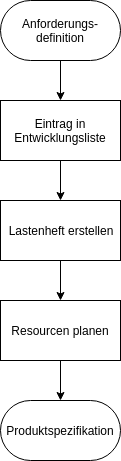
\includegraphics[keepaspectratio,height=0.8\textwidth]{images/3_2_1_1_Anforderungsdefinition_redraw.png}
  \caption[Anforderungsdefinition bis Produktspezifikation]{Die nötigen Tätigkeiten von der Anforderung bish zur Produktspezifikation.}
  \label{fig:Anforderungsdefinition}
\end{figure}

Es findet in diesem Schritt eine erste Bewertung des entsprechenden Entwicklungsvorschlags statt. Diese wird priorisiert und in die Entwicklungsliste eingetragen. Der Vorschlag wird danach in Form eines Lastenheftes dokumentiert und Ressourcen werden verplant. Hier kann es zu Verschiebungen von bereits priorisierten Entwicklungsprojekten kommen.

\section{Produktspezifikation}

Der \ac{TPL} leitet ein oder mehrere Workshops in denen die Anforderungen aus dem Lastenheft des \ac{PD} in Soft- und Hardware-Anforderungen ins Pflichtenheft umgesetzt werden. Dies geschieht mit der Unterstützung vom \ac{BDE} und \ac{BPI}. Die Gliederung der Anforderungen und die Zuordnung zu Soft bzw. Hardware-Subsystemen kann durch eine Use-Case-Analyse erfolgen.

Bei der Erstellung des Pflichtenhefts sollen möglichst Synergien der Soft- und Hardwarekomponenten genützt und die Möglichkeiten neuer Informationstechnologien ausgeschöpft werden. 

\begin{figure}[h]
    \centering
    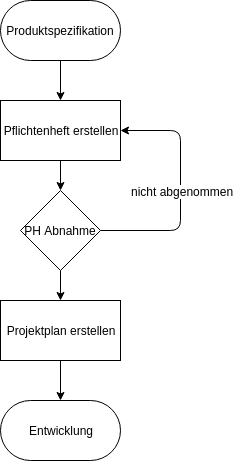
\includegraphics[keepaspectratio,height=0.8\textwidth]{images/3_2_1_2_Produktspezifiktation_redraw.png}
    \caption[Produktspezifikation bis Systemdesign]{Die nötigen Tätigkeiten von der Produktspezifikation bis zum Systemdesign.}
    \label{fig:Produktspezifiktation}
  \end{figure}

Sobald das Pflichtenheft erstellt wurde, wird ein Projektplan erstellt, um folgende Punkte zu definieren:

\begin{itemize}

    \item Abschätzung des Gesamtumfanges, -aufwandes und der Gesamtkosten
    \item Meilensteine 
    \item Iterationen und deren Ziele in den Phasen
    \item Zeitplan und Budget
    \item Zur Verfügung stehende Kapazitäten 
    \item Notwendige Aktivitäten für den korrekten Abschluss

\end{itemize}

Die Projektplanung erfolgt wiederum im Rahmen von ein oder mehreren Workshops. In diesen schätzt der \ac{TPL} mit Unterstützung durch die \ac{BDE}, \ac{BPI} und \ac{PD} den Aufwand, um das Projekt umsetzen zu können, und entwickelt einen Terminplan, der die Rahmenbedingungen des Projekts erfüllt.

Weiters werden die Meilensteine der Projektphasen festgelegt, an denen der Projektfortschritt beurteilt und die Aufwände und Kosten geprüft werden. Auf der Basis der Aufwandsschätzung und des Terminplans werden die benötigten Ressourcen definiert, um das Projekt umzusetzen. Der \ac{TPL} legt fest, welche Rollen und wie viele Ressourcen in welcher Projektphase benötigt werden.

Schließlich erstellt der \ac{TPL} einen Plan für die ordentliche Übergabe des Projekts und definiert die damit verbundenen Aktivitäten. Damit kann in die Entwicklungsphase übergegangen werden.

\section{Entwicklungs-Start}

Der Entwicklung-Start Prozess stellt sicher, dass in der nächsten Phase, der Entwicklungs-Umsetzung, alle notwendigen Informationen vorliegen und die Infrastruktur bereitsteht. 
Folgende Aspekte werden berücksichtigt:

\begin{itemize}
    \item Qualitätsüberprüfung der Anforderungen
    \item Bestimmung der Systemgrenzen
    \item Validierung der Aufwandsschätzung
    \item Abarbeitungsplan (Releaseplan)
    \item Ziele der Testung
    \item Überprüfung der Infrastruktur
\end{itemize} 

\subsection{Anforderungsreview}

Anforderungen wurden durch die \ac{PD} definiert. Vor der Entwicklungs-Umsetzung werden diese zu einem Termin von \ac{EPL}, Software Architekten und gegebenenfalls einzelnen Personen des Entwicklungsteams reviewed. 3 Aspekte sind zu klären:

\paragraph{Verständlichkeit:} 
Die Anforderungen müssen soweit klar, verständlich und widerspruchsfrei sein.

\paragraph{Umsetzbarkeit:} 
Die Anforderungen sind auf ihre technische Umsetzbarkeit hin zu überprüfen.

\paragraph{Vereinfachung:} 
Es ist zu klären, ob eine Änderung der Anforderungsbeschreibung die technische Umsetzung vereinfachen würde.

\subsection{Systemdesign erstellen}

Es werden die Systemgrenzen zu anderen Produkten des Unternehmens und externen zugekauften Produkten definiert. Daraus ergeben sich Schnittstellen zu den besagten Produkten. Diese Phase wird vorrangig von \ac{EPL}s oder Enterprise-Architekten vollzogen, kann jedoch auch von den Software-Architekten umgesetzt werden.

\subsection{Entwicklungs-Aufwände bestimmen}

Die Anforderungen sind bezüglich der Entwicklungs-Aufwände zu bewerten. Gemeinsam mit den geplanten Aufwänden für Koordination, Dokumentation, Tests, etc. sind die gesamten Entwicklungs-Aufwände grob zu planen.

\subsection{Release Planung}

Die geplanten Releases (Gruppierung von Anforderungen) sind mit Start-Datum und Ende-Datum zu definieren.
Die Zuteilung der Anforderungen zu Releases erfolgt gemeinsam mit dem Produktmanagement und der Software Entwicklung. Hier ist zu beachten, dass Releases in sinnvoller technischer Reihenfolge abgewickelt werden sollten. Weiters müssen die zur Verfügung stehenden Ressourcen bedacht werden.

\subsection{Entwicklungs-Infrastruktur erstellen}

In Abhängigkeit vom Systemdesign und dem gewählten Inventar an Umsetzungsmechanismen erstellt der \ac{EPL} bzw. der Architekt einen Plan für die Entwicklungsumgebung(en) und Testumgebung, in denen die Umsetzung erfolgt. Darin enthalten ist die Auswahl der Hardware- und Software-Komponenten sowie die nötige Infrastruktur (Build-Umgebung, Datenbank, Versionierung, Entwicklungsumgebung, etwaige andere Tools).

\section{Entwicklungs-Umsetzung}

Für die relevanten Anforderungen werden Design-Entscheidungen getroffen, Testfälle definiert, auf Basis des Designs implementiert, Testfälle durchgeführt und das Release ausgeliefert.

Dies wird in einem iterativem Verfahren abgehandelt, angelehnt an das Scrum Konzept werden Sprints definiert, um die Umsetzung voranzutreiben.

\subsection{Sprint}

Die Arbeit erfolgt in Iterationen von bis zu einem Monat. Jeder abgeschlossene Sprint soll einen konkreten Wert für den Kunden oder Benutzer erstellt haben. Die Länge des Sprints sollte konsistent bleiben. \parencite[vgl.][S. 62]{Rubin:2012}

Die Sprintplannung erfolgt zu einem Termin, an dem über den Inhalt und die Umsetzungsdetails beraten wird. \parencite[vgl.][S. 339]{Rubin:2012} Zu diesem Zeitpunkt werden auch Testfälle spezifiziert.

\subsection{Release-Übergabe und Abnahme}

Die fertige Software wird an das Produktmanagement bzw. den Produktverantwortlichen übergeben. Der Umfang der Software ist in den Release-Notes dokumentiert. Diese beinhalten zumindest die umgesetzten Anforderungen, die behobenen Fehlerfälle, neu eingeführte Parameter und ggf. bekannte Probleme. 

Das Produktmanagement bzw. den Produktverantwortlichen prüft gemeinsam mit der Entwicklung die übergebene Release anhand der Anforderungen und prüft die übergebene Dokumentation. Werden die Anforderungen erfüllt, ist die Entwicklung abgenommen und somit freigegeben; falls nicht alle Anforderungen erfüllt werden, muss die Entwicklung die fehlenden oder nicht fehlerfreien Teile nachliefern.

\subsection{Produkt Schulung}

Bei Bedarf (initiiert von den Produktmanagern bzw. dem Produktverantwortlichen) werden die neuen Features vorgestellt und die Anwender (Projekt-Entwickler, bzw. -Abwickler) geschult.

\subsection{Produkt Review}
Nach dem ersten Einsatz der Release kann eine Produkt Review eingeleitet werden. Ziel ist es, für zukünftige Projekte, Verbesserungspotential zu finden.

\section{System-Test}

Ein Mitarbeiter des Bereiches \ac{BDE} bzw. \ac{BPI} testet die aus der Umsetzung entstandene Software zusammen mit allen notwendigen Fremdgewerken entsprechend des Testplans und füllt die Testprotokolle mit den gewonnen Ergebnissen aus. Entscheidend dabei ist, dass im Test entstandene Fehler auf ihre Reproduzierbarkeit überprüft werden. Eventuell muss der Testplan entsprechend angepasst werden, damit der Entwickler in der Lage ist, den Fehler zu reproduzieren und zu beseitigen.

\begin{figure}[h]
    \centering
    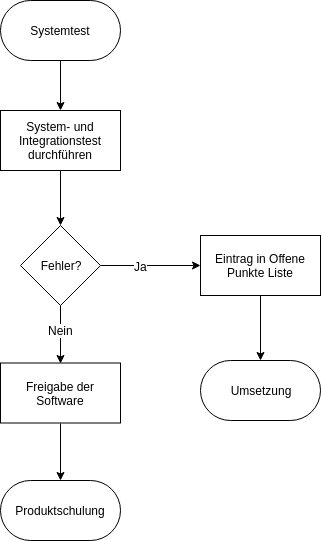
\includegraphics[keepaspectratio,height=0.9\textwidth]{images/3_2_1_5_Systemtest_redraw.png}
    \caption[Systemtest]{Der Ablauf der Systemtests.}
    \label{fig:Produktspezifiktation}
\end{figure}

\section{Produkt-Schulung}

Der \ac{TPL} organisiert für jede Zielgruppe (\ac{BPI}, \ac{PD}) ein oder mehrere Workshops, in denen von der \ac{BDE} bzw. \ac{BPI} die Anwendung der Software mithilfe der erstellten Unterlagen geschult wird. Die Teilnehmer dieser Workshops sind dann in der Lage, die notwendigen Tätigkeiten für das Produkt-Rollout durchzuführen und können die End-Anwender schulen.



\chapterend